\section{Лекция 31} 
{\tiny Если какие-то части выглядят слишком вырвиглазно и нечитабельно и у вас есть идеи как это исправить, пишите @nih3kwo/создавайте ишью или пуллрек}

Напоминание: $V, W$ --- два векторых пространства над полем $F$ 

$\phi \colon V \mapsto W$ --- линейное отображение, $r = \rk(\phi) \implies \exists$ базис $\E$ в $V$ и базис $\F$ в $W$, такие что 
\begin{equation*}
    A(\phi, \E, \F) = \left(
        \begin{array}{c|c}
            E & 0 \\
            \hline
            0 & 0
        \end{array}
    \right)
\end{equation*}

где $r$ --- количество единиц.

\subsection{Теорема о сингулярных базисах}
Пусть 
\begin{math}
    \begin{aligned}[t]
        &\EE \text{ --- евклидово пространство со скалярным произведением } (\bigcdot, \bigcdot), \quad \dim \EE = n, \\
        &\EE \text{ --- другое евклидово пространство со скалярным произведением } (\bigcdot, \bigcdot)', \quad \dim \EE' = m, \\
        &\phi \colon \EE \to \EE' \text{ --- линейное отображение}, r = \rk \phi (= \dim \Im \phi) 
    \end{aligned}
\end{math}

\begin{theorem}
    Существуют ортонормированные базисы $\E$ в $\EE$ и $\F$ в $\FF$, такие что
    \begin{equation*}
        \label{lec31:SVD_matrix}
        A(\phi, \E, \F) =
        \resizebox{6cm}{!}{
            \begin{math}
                \begin{blockarray}{cccccccccc}
                    \begin{block}{(ccccc|ccccc)}
                        \sigma_{1} & 0 & 0 & \dots & 0 & & & &\\
                        0 & \sigma_{2} & 0 & \dots & 0 & & & &\\
                        0 & 0 & \sigma_{3} & \dots & 0 & & & \scaleobj{2}{0} & &\\
                        \vdots & \vdots & \vdots & \ddots & \vdots &\\
                        0 & 0 & 0 & \dots & \sigma_{r} &\\
                        \cline{1-10}
                        & & & & & & & & &\\
                        & & & & & & & & &\\
                        & & \scaleobj{2}{0} & & & & & \scaleobj{2}{0} & &\\
                        & & & & & & & & &\\
                        & & & & & & & & &\\
                    \end{block}
                \end{blockarray}
            \end{math}
        }
        = \Sigma
    \end{equation*}

    где $\sigma_{1} \geq \sigma_{2} \geq \dots \geq \sigma_{r} > 0$

    Более того, числа $\sigma_{1}, \dots, \sigma_{r}$ определены однозначно.
\end{theorem}

\begin{proof}
    \begin{description}
        \item[Существование:] \mbox{}

        Пусть $\phi^{*} \colon \EE' \to \EE$ --- линейное отображание, сопряженное к $\phi$. Положим $\psi := \phi^{*} \cdot \phi$. Тогда $\psi$ --- линейный оператор на $\EE$.

        $\forall x, y \in \EE \quad (x, \psi(y)) = (x, \phi^{*} \phi(y)) = (\phi(x), \phi(y))'$

        В частности, $(x, \psi(y)) = (\psi(x), y) \implies \psi = \psi^{*}.$
    
        Тогда $\exists$ ортнонормированный базис $\E = (e_1, \dots, e_n)$ в $\EE$, такой что $A(\psi, \E) = \diag(s_1, s_2, \dots, s_n)$. Тогда $\forall i = 1, \dots, n$ имеем
        \begin{equation*}
            \left.
                \begin{aligned}
                (e_i,\psi(e_i)) &= (\phi(e_i),\phi(e_i))' &\geq 0 \\
                (e_i,\psi(e_i)) &= (e_i, s_i e_i) = s_i(e_i,e_i) &= s_i
                \end{aligned}
            \right|
                \implies s_i \geq 0
        \end{equation*}

        Переставив векторы в $\E$, добьёмся того, что $s_1 \geq s_2 \geq \dots \geq s_n \geq 0.$

        Пусть $k \in \{1, \dots, n\}$ таково, что $s_k > 0, s_{k+1} = 0$. Тогда $\forall i \geq k+1$ имеем $0 = s_i = (\phi(e_i), \phi(e_i))' \implies \phi(e_i) = 0 \implies e_i \in \ker \phi$
        
        $\forall i = 1, \dots, k$ положим $\sigma_i = \sqrt{s_i}$ и $f_i = \frac{1}{\sigma_i} \phi(e_i)$. Тогда $\forall i, j = 1, \dots, k$ имеем

        \begin{align*}
            &(f_i, f_j)' = (\frac{1}{\sigma_i} \phi(e_i), \frac{1}{\sigma_j} \phi(e_j)) = \frac{1}{\sigma_i \sigma_j} (\phi(e_i), \phi(e_j)) =  \frac{1}{\sigma_i \sigma_j} (e_i, \phi^{*} \phi (e_j)) = \\
            &=  \frac{1}{\sigma_i \sigma_j} (e_i, \psi(e_j)) =  \frac{1}{\sigma_i \sigma_j} (e_i, (\sigma_j)^2 e_j ) =  \frac{\sigma_j}{\sigma_i} (e_i, e_j) = \delta_{i j} =
            \begin{cases}
                1, &i = j, \\
                0, &i \neq j.
            \end{cases}
        \end{align*}
        Итого: $f_1, \dots, f_k$ --- ортонормированная система в $\EE'$. Дополним эту систему до ортонормированного базиса $\F = (f_1, \dots, f_m)$ в $\EE'$.

        Тогда в $A(\phi, \E, \F)$:
        \begin{itemize}
            \item $i = 1, \dots, k \colon \phi(e_i) = \sigma_i f_i$
            \item $i \geq k + 1 \colon \phi(e_i) = 0$
        \end{itemize}

        Что и даёт нам \hyperref[lec31:SVD_matrix]{искомый вид} матрицы

        \bigskip
        Отсюда, в частности $\rk \phi = k \implies k = r$.

        \item[Единственность:] \mbox{}
        \item[] 
            Если $\E$ и $\F$ в $\EE$ и $\EE'$ и $A(\phi, \E, \F)$ имеет вид \hyperref[lec31:SVD_matrix]{$\Sigma$}, то $A(\psi, \E) = \Sigma^{T} \Sigma = \diag(\sigma_1^2, \dots, \sigma_r^2, 0, \dots, 0) $
            
            $\implies \sigma_1^2, \dots, \sigma_r^2$ --- ненулевые собственные значения оператора $\psi \implies$ они определены однозначно.
 
    \end{description}

    \bigskip    
    \begin{definition}
        В условиях теоремы базисы $\E$ и $\F$ называются \textit{сингулярными базисами}, 
        
        векторы $e_i, f_j$ называются \textit{сингулярными векторами}, 
        
        числа $\sigma_1, \dots, \sigma_r$ --- \textit{сингулярныеми значениями} линейного отображения $\phi$
    \end{definition}

    \begin{comment}
        \begin{enumerate} 
            \item Базисы $\E$ и $\F$ определены, вообще говоря, неоднозначно.
            \item Доказательство теоремы даёт алгоритм нахождения сингулярных значений и сингулярных базисов.
            \item Если $\E$ и $\F$ --- сингулярные базисы для линейного отображения $\phi$ и $A(\phi, \E, \F) = $ \hyperref[lec31:SVD_matrix]{$\Sigma$}, то $\E$ и $\F$ --- сингулярные базисы для линейного отображения $\phi^{*} = A(\phi, \F, \E) = \Sigma^T$
        \end{enumerate}
    \end{comment}

    \textbf{Свойства сингулярных базисов}:
    \begin{enumerate}
        \item 
            $\phi(e_i) = \begin{cases}
            \frac{1}{\sigma_i} f_i, & i \leq r \\
            0, & i > r
            \end{cases} \qquad 
            \phi^{*}(f_i) = \begin{cases}
                \frac{1}{\sigma_i} e_i, & i \leq r \\
                0, & i > r
            \end{cases}$

        \item $\forall i = 1, \dots, n$, вектор $e_i$ --- собственный вектор линейного оператора $\phi^{*} \phi$ с собстенным значеним $\sigma_i^2$
        
        $\forall j = 1, \dots, m$, вектор $f_j$ --- собственный вектор линейного оператора $\phi \phi^{*}$ с собственным значением $\sigma_i^2$

        \item $\sigma_1^2, \dots, \sigma_r^2$ --- в точности все ненулевые собственные значения линейного оператора $\phi^{*} \phi$, а также $\phi \phi^{*}$

    \end{enumerate}
\end{proof}

\subsection{Сингулярное разложение матрицы и её сингулярные значения}

\begin{corollary}
    Из SVD: Пусть $A \in \text{Mat}_{m \times n}(\RR), \rk A = r \implies \exists$ ортогональные матрицы $U \in M_m (\RR)$ и $V \in M_n (\RR)$, такие что 
    \begin{equation*}
        A = U \Sigma V^T
    \end{equation*}
    где $\Sigma$ --- матрица из \hyperref[lec31:SVD_matrix]{теоремы}, $\qquad \sigma_1 \geq \dots \geq \sigma_r > 0$. Более того, числа $\sigma_1, \dots, \sigma_r$ определны однозначно.
\end{corollary}

\begin{proof}
    Применяем теорему к линейному отображению $\phi \colon \RR^n \to \RR^m, x \mapsto   A x$

    $\exists$ ортогональные матрицы $U \in M_n (\RR), V \in M_m (\RR)$, такие что
    \begin{equation*}
        U^{-1} A V = \hyperref[lec31:SVD_matrix]{\Sigma}, \quad  \sigma_1 \geq \dots \geq \sigma_r > 0 \implies A = U \Sigma \underbracket{V^{-1}}_{\text{ортог.} = V^T}
    \end{equation*}
\end{proof}

\subsection{Усечённое сингулярное разложение матрицы}

%простите за ужас ниже... Просто раз уже это было написано на доске Авдеевым, наверное не писать это тоже было бы плохо...

$\underset{\scriptscriptstyle{m \times n}}{\widehat{A}} = \underset{\scriptscriptstyle{m \times m \ }}{U} \underset{\scriptscriptstyle{m \times n \ }}{\Sigma} \underset{\scriptscriptstyle{n \times n}}{V^T}$ --- сингулярное разложение для $A$

$u_i$ --- $i$-ый столбец матрицы $U$

$v_j$ --- $j$-ый столбец матрицы $V$

\begin{proposal}
    \begin{enumerate}
        \item Если $m \leq n$, то $A = \underset{\scriptscriptstyle{m \times m \ }}{\widehat{U}} \underset{\scriptscriptstyle{m \times m \ }}{\widehat{\Sigma}} \underset{\scriptscriptstyle{m \times n}}{\widehat{V}^T}$, 
        
        где  $\widehat{U} = U, \ \widehat{\Sigma} = $
        \resizebox{3.5cm}{!}{
            \begin{math}
                \begin{pmatrix} 
                    \sigma_1 & \dots & 0 & \dots & 0 \\
                    \vdots & \ddots & \vdots & \dots & \vdots \\
                    0 & \dots & \sigma_r & \dots & 0 \\
                    \vdots & \vdots & \vdots & \ddots & \vdots \\
                    0 & \dots & 0 & \dots & 0
                \end{pmatrix}
            \end{math}
        }
        $ = \diag(\sigma_1, \dots, \sigma_r, \dots, 0) \in M_n(\RR), \ \widehat{V} = (v_1, \dots, v_m) $
        \item Если $m \geq n$, то $A = \underset{\scriptscriptstyle{m \times n \ }}{\widehat{U}} \underset{\scriptscriptstyle{n \times n \ }}{\widehat{\Sigma}} \underset{\scriptscriptstyle{n \times n}}{\widehat{V}^T}$,
        
        где $\widehat{U} = (u_1, \dots, u_n), \ \widehat{\Sigma} = \diag(\sigma_1, \dots, \sigma_r, 0, \dots, 0) \in M_n(\RR), \ \widehat{V} = V $.
    \end{enumerate}

\end{proposal}


\begin{proof}
    \begin{enumerate}
        \item 
        \begin{math}
            A = 
            \overbracket{\left(
                \begin{array}{ccc}
                    \star & \dots & \star \\
                    \vdots & \ddots & \vdots\\
                    \star & \dots & \star
                \end{array}
            \right)}^{U}
            \cdot
            \overbracket{\left(
                \begin{array}{ccc|c}
                    \star & \dots & \star & \\
                    \vdots & \ddots & \vdots & \scaleobj{2}{0}\\
                    \star & \dots & \star & 
                \end{array}
            \right)}^{\Sigma}
            \cdot
            \overbracket{\left(
                \begin{array}{ccc}
                    \star & \dots & \star\\
                    \vdots & \ddots & \vdots\\
                    \star & \dots & \star\\
                    \hline
                    & &\\
                    &  \scaleobj{2}{\star} &
                \end{array}
            \right)}^{V^T}
        \end{math}

        \begin{equation}
            \Sigma \cdot V^T = \widehat{\Sigma} \cdot \widehat{V}^T \implies U \Sigma V^T = \widehat{U} \widehat{\Sigma} \widehat{V}^T
        \end{equation}

        \item 
        \begin{math}
            A = 
            \overbracket{\left(
                \begin{array}{ccc|c}
                    \star & \dots & \star &  \\
                    \vdots & \ddots & \vdots &  \scaleobj{2}{\star}\\
                    \star & \dots & \star & 
                \end{array}
            \right)}^{U}
            \cdot
            \overbracket{\left(
                \begin{array}{ccc}
                    \star & \dots & \star\\
                    \vdots & \ddots & \vdots\\
                    \star & \dots & \star\\
                    \hline
                    & &\\
                    &  \scaleobj{2}{0} &
                \end{array}
            \right)}^{\Sigma}
            \cdot
            \overbracket{\left(
                \begin{array}{ccc}
                    \star & \dots & \star\\
                    \vdots & \ddots & \vdots\\
                    \star & \dots & \star\\
                \end{array}
            \right)}^{V^T}
        \end{math}

        \begin{equation*}
            U \cdot \Sigma = \widehat{U} \cdot \widehat{\Sigma} \implies U \Sigma V^T = \widehat{U} \widehat{\Sigma} \widehat{V}^T
        \end{equation*}
    \end{enumerate}
\end{proof}

\begin{definition}
    Разложение $A = \widehat{U} \widehat{\Sigma} \widehat{V}^T$ называется \emph{усечённым сингулярным разложением матрицы} $A$.
\end{definition}

\begin{proposal}
    Матрица $A$ представима в виде:
    \begin{equation*}
        A = u_1 \sigma_1 v_1^T + u_2 \sigma_2 v_2^T + \dots + u_r \sigma_r v_r^T \text{\customlabel{lec31:star}{($\star$)}}
    \end{equation*}
    где $r = \rk A, \rk (u_i \sigma_i v_i^T) = 1.$
\end{proposal}

\begin{proof}
    \begin{equation*}
        A = \widehat{U} \widehat{\Sigma} \widehat{V}^T = \begin{pmatrix} u_1 & u_2 & \dots \end{pmatrix} 
        \begin{pmatrix} 
            \sigma_1 & \dots & 0 \\
            \vdots & \ddots & \vdots \\
            0 & \dots & \sigma_r
        \end{pmatrix}
        \begin{pmatrix} v_1^T \\ \\ v_2^T\\ \vdots \end{pmatrix} = \begin{pmatrix} u_1 & u_2 & \dots \end{pmatrix} 
        \begin{pmatrix} \sigma_1 v_1^T \\ \\ \sigma_2 v_2^T \\ \dots \\ \sigma_r v_r^T \\ 0 \\ \dots \\ 0 \end{pmatrix}
        = u_1 \sigma_1 v_1^T + \dots + u_r + \sigma_r + v_r^T
    \end{equation*}
\end{proof} 

\begin{comment}
    Для хранения матрицы $A$ в виде \ref{lec31:star} требуется $mr + r + nr = (m + n + 1) \cdot r$ памяти вместо $m \cdot n$
\end{comment}


\subsection{Фробениусова норма матрицы, её инвариантность относительно умножения на ортогональную матрицу слева или справа}

Напоминание $\text{Mat}_{m \times n} (\RR)$ --- евклидово пространство со скалярным произведением $(A, B) = \tr (A^T, B)$. В этом евклидовом пространства ``длина'' матрицы называется её нормой Фробениуса (или фробениусовой нормой), обозначается как $\norm{A}$.

\begin{equation*}
    \norm{A} = \sqrt{\tr (A^T A)} = \sqrt{\tr (A A^T)} = \sqrt{\sum_{i=1}^m \sum_{j=1}^n a_{i j}^2}
\end{equation*}

\begin{example}
    $u \in \RR^m, v \in \RR^n, |u| = |v| = 1 \implies \forall \sigma > 0$
    \begin{equation*}
        \norm{u \sigma v^T}^2 = \tr (v \sigma \underbracket{u^T \cdot u}_{=1} \sigma v^T ) = \sigma^2 \cdot \tr (v v^T) = \sigma^2 \cdot \tr (\underbracket{v^T \cdot v}_{=1}) = \sigma^2 \implies \norm{u \sigma v^T} = \sigma
    \end{equation*}
\end{example}

\begin{proposal}
    $\forall A \in \text{Mat}_{m \times n}, \forall$ ортогональных матриц $U \in M_m (\RR), V \in M_n (\RR)$ верно $\norm{U A V} = \norm{A}$, то есть норма фробениуса инвариантна относительно умножения слева или справа на ортогональные матрицы.
\end{proposal}

\begin{proof}
    \begin{equation*}
        \norm{U A V}^2 = tr(V^T \cdot A^T \underbracket{U^T \cdot U}_{=E} \cdot A \cdot V) = \tr (V^T \cdot A^T \cdot A \cdot V) = \tr (A^T \cdot A \cdot \underbracket{V \cdot V^T}_{=E}) = \tr (A^T A) = \norm{A}^2
    \end{equation*}
\end{proof}

\subsection{Теорема Эккарта-Янга о низкоранговом приближении}

\begin{theorem}
    Пусть $A \in \text{Mat}_{m \times n}, \rk A = r$
    
    $A = U \cdot \Sigma \cdot V^T$ --- сингулярное разложением для $A$.

    Тогда $\forall k < r$ минимум величины $\norm{A - B}$ среди всех матриц $B \in \text{Mat}_{m \times n} (\RR)$ с условием $\rk B \leq k$ достигается при 
    
    \begin{equation*}
        B = U \cdot \Sigma_k \cdot V^T, \quad \text{где } \Sigma_k = 
        \resizebox{6.5cm}{!}{
            \begin{math}
            \begin{blockarray}{ccccccccccc}
                \begin{block}{(cccccc|ccccc)}
                \sigma_{1} & \dots & 0 & 0 & \dots & 0 & & & & &\\
                \vdots & \ddots & \vdots & \vdots & \ddots & \vdots & & & & &\\
                0 & \dots & \sigma_{k} & \vdots & \dots & 0 & & \scaleobj{2}{0} & & &\\
                0 & \dots & \dots & 0 & \dots & 0 & & & & &\\
                \vdots & \ddots & \vdots & \vdots & \ddots & \vdots & & & & &\\
                0 & \dots & 0 & 0 & \dots & 0 & & & & &\\
                \cline{1-11}
                & & & & & & & & & &\\
                & & & & & & & & & &\\
                & & \scaleobj{2}{0} & & & & & \scaleobj{2}{0} & & &\\
                & & & & & & & & & &\\
                & & & & & & & & & &\\
                \end{block}
            \end{blockarray}
            \end{math}
            }
    \end{equation*}
    (То есть мы обнуляем все значения $\Sigma$ после $k$).
\end{theorem}

\begin{lemma}
    \label{lec31:lemma_1}
    Пусть $a_1, \dots, a_p$ --- ортонормированная система векторов некоторого евклидового пространства $\EE$ и пусть $S = \langle a_1, \dots, a_p \rangle$. Тогда $\forall b \in \EE$ 
    \begin{equation}
        |\pr_S b|^2 = (b, a_1)^2 + \dots + (b, a_p)^2.
    \end{equation}
    В частности, если $b \in S$, то $|b|^2 = (b, a_1)^2 + \dots + (b, a_p)^2$, так как если $b \in S$, то $\pr_S b = b$.
\end{lemma}

\begin{proof}
    \begin{equation*}
        |\pr_S b|^2 = | (b, a_1) a_1 + \dots + (b, a_p) a_p |^2 = \text{(теорема Пифагора)} = (b, a_1)^2 \cdot \underbracket{|a_1|^2}_{=1} + \dots + (b, a_p)^2 \cdot \underbracket{|a_p|^2}_{=1} = (b, a_1)^2 + \dots + (b, a_p)^2
    \end{equation*}
\end{proof}

\begin{lemma}
    \label{lec31:lemma_2}
    (Техническая лемма)

    Пусть $s_1, \dots, s_r, t_1, \dots, t_r \in \RR$.

    $s_1 \geq s_2 \geq \dots \geq s_r > 0$

    $0 \leq t_i \leq 1 \quad \forall i = 1, \dots, r$

    $t_1 + \dots + t_r \geq r - k$ для некоторого $k \leq r$. Тогда 

    \begin{equation*}
        s_1 t_1 + \dots + s_r t_r \geq s_{k+1} + \dots + s_r.
    \end{equation*}
\end{lemma}

\begin{proof}
    \begin{description}
        \item[``На пальцах'':] \mbox{}
        \begin{center}
            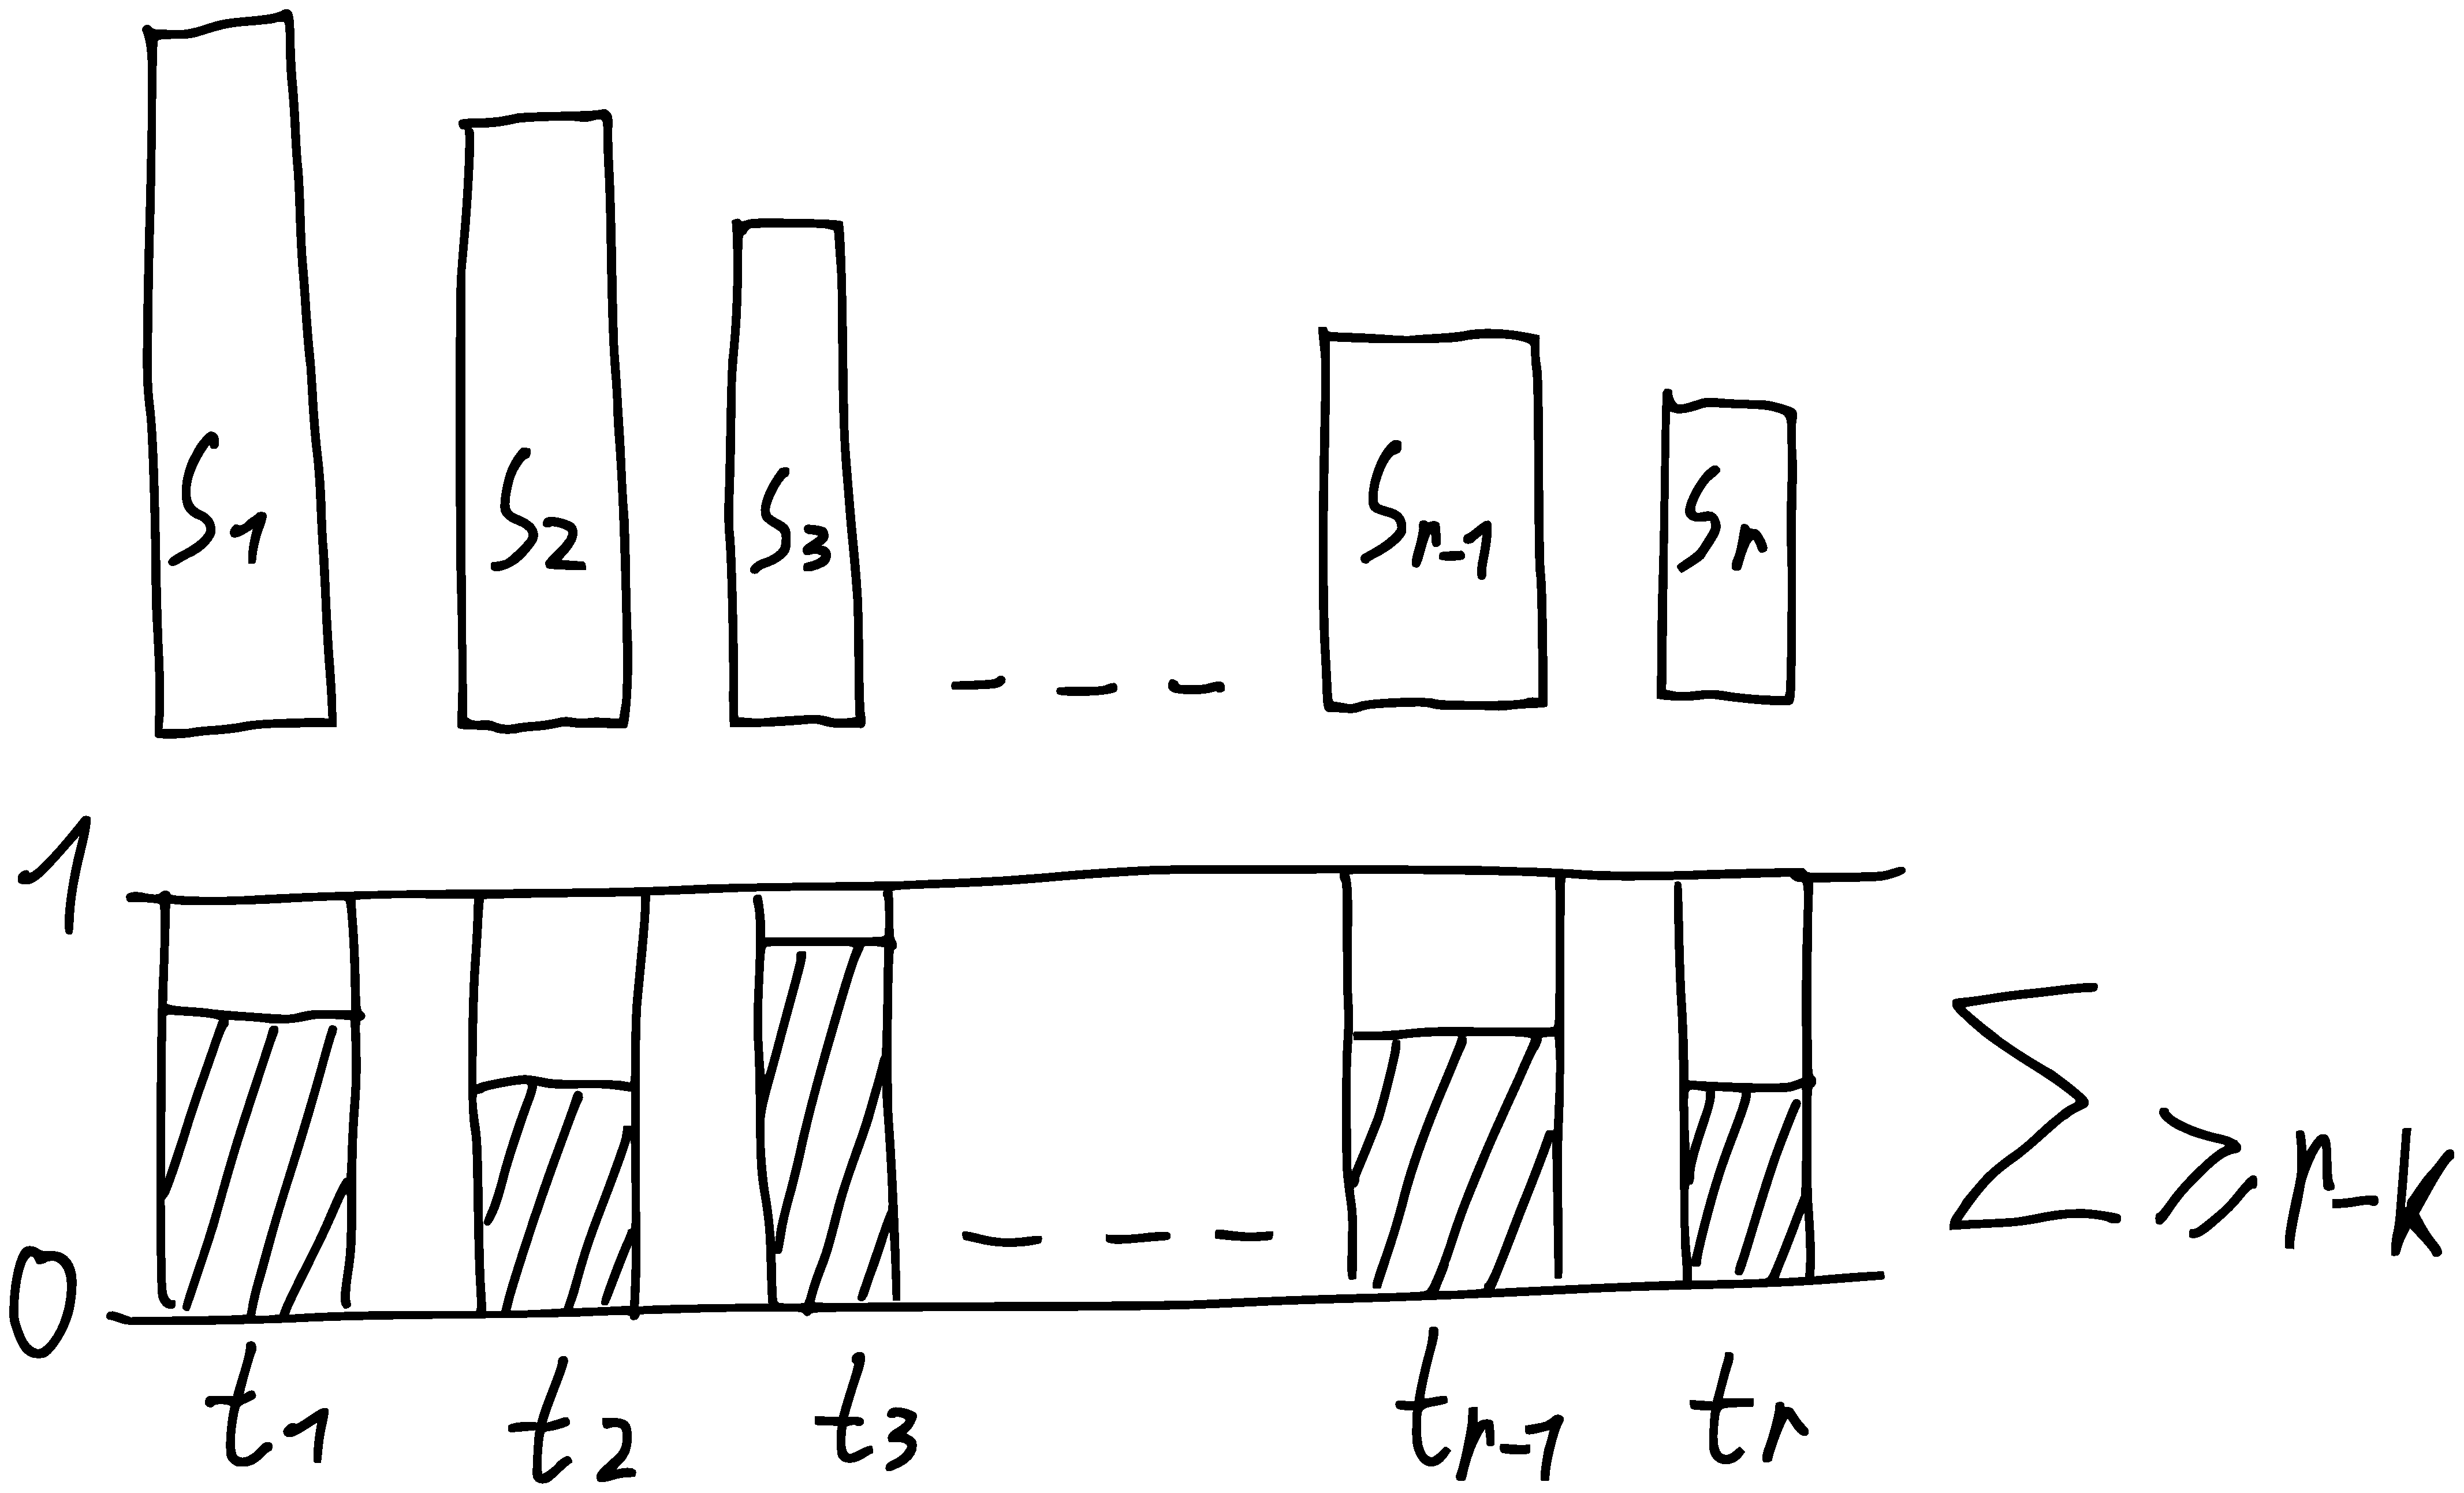
\includegraphics[height=6cm]{img/lecture31_drawing_1}
        \end{center}

        Будем считать сумму как умножение нижней ``колбы'' $0 \leq t_i \leq 1$ на значение сверху $s_i$. То есть изначальная сумма это:
        \begin{equation*}
            s_1 t_1 + \dots + s_{r-1} t_{r-1} + s_r t_r
        \end{equation*}

        Посмотрим на последнюю колбу $t_r$. Если она не полна, возьмем и ``перельем'' в неё содержимое первой колбы так, чтобы она ``заполнилась''. Если она последняя колба не заполнилась от переливания первой, прибаваляем следующие за первой.
        
        Такое переливание уменьшает сумму, так теперь вместо умножения больше $s_1$ на $t_1$ мы будем умножать меньшую $s_r$ на это же $t_1$ перелитое в $t_r$.

        После ``заполнения'' $t_r$, то есть когда она станет равна 1, начинаем таким же образом заполнять $t_{r-1}$ и т.д. Условие гарантирует нам то, что последние $r - k$ колб будут заполнены полностью. Итого, так как полные колбы имеют значение 1, у нас в сумме точно будет будет хотя бы:
        \begin{equation*}
            s_r \cdot 1 + \dots + s_{k+1} \cdot 1. 
        \end{equation*}

        А это в свою очередь по построению меньше изначальной суммы. Это и даёт нам доказываемое неравенство.
        \item[Формальное доказательство со слайдов:] \mbox{}
    
            Индукция по $r$ при фиксированном $k$. При $r = k$ всё верно.

            Пусть теперь $r > k$, так что $r - k \geq 1$.

            По условию имеем $t_1 + \dots + t_{r-1} \geq r - k - t_r \geq 1 - t_r$, поэтому можно подобрать такие числа $\delta_1, \dots, \delta_r$, что 
            \begin{equation*}
                0 \leq \delta_1 \leq t_1, \dots, 0 \leq \delta_{r-1} \leq t_{r-1}  \text{ и } \delta_1 + \dots + \delta_{r-1} = 1 - t_r.
            \end{equation*}
            Для каждого $i = 1, \dots, r-1$ положим $t'_i = t_i - \delta_i$, тогда $0 \leq t'_i \leq 1$. Имеем
            \begin{equation*}
                t'_1 + \dots + t'_{r-1} = t_1 + \dots + t_r - \delta_1 - \dots - \delta_{r - 1} - t_r \geq (r-1) - k
            \end{equation*}
            и тогда по предположению индукции получаем
            \begin{align*}
                & s_1 t'_1 + \dots s_{r-1} t'_{r-1} \geq s_{k+1} + \dots + s_{r-1}, \text{ откуда} \\
                & s_1 t_1 + \dots + s_r t_r = s_1 (t'_1 + \delta_1) + \dots + s_{r-1} (t'_{r-1} + \delta_{r-1}) + s_r t_r = \\
                & = s_1 t'_1 + \dots s_{r-1} t'_{r-1} + s_1 \delta_1 + \dots + s_{r-1} \delta_{r-1} + s_r t_r \geq \\
                & \geq s_1 t'_1 + \dots s_{r-1} t'_{r-1} + s_r (\delta_1 + \dots + \delta_{r-1} + t_r) = \\
                & = s_1 t'_1 + \dots s_{r-1} t'_{r-1} + s_r \geq + s_{k+1} + \dots + s_{r-1} + s_r.
            \end{align*}
    \end{description}
\end{proof}

\begin{proof}[Доказательство теоремы]~
    Так как $\norm{A}$ инвариантна относительнто умножения на ортогональную матрицу слева и справа, достаточно доказать утверждение для случая $A = \Sigma$. Тогда при $B = \Sigma_k$ получаем
    \begin{equation*}
        \norm{\Sigma - B}^2 = \norm{
            \resizebox{5cm}{!}{
                \begin{math}
                \begin{blockarray}{ccccccccccc}
                    \begin{block}{(cccccc|ccccc)}
                    0 & \dots & 0 & 0 & \dots & 0 & & & & &\\
                    \vdots & \ddots & \vdots & \vdots & \ddots & \vdots & & & & &\\
                    0 & \dots & 0 & \vdots & \dots & 0 & & \scaleobj{2}{0} & & &\\
                    0 & \dots & \dots & \sigma_{k+1} & \dots & 0 & & & & &\\
                    \vdots & \ddots & \vdots & \vdots & \ddots & \vdots & & & & &\\
                    0 & \dots & 0 & 0 & \dots & \sigma_r & & & & &\\
                    \cline{1-11}
                    & & & & & & & & & &\\
                    & & & & & & & & & &\\
                    & & \scaleobj{2}{0} & & & & & \scaleobj{2}{0} & & &\\
                    & & & & & & & & & &\\
                    & & & & & & & & & &\\
                    \end{block}
                \end{blockarray}
                \end{math}
            }    
        }^2
        = \sigma_{k+1}^2 + \dots + \sigma_r^2
    \end{equation*}

    Пусть теперь $B \in \text{Mat}_{m \times n} (\RR)$ --- произвольная матрица у словием $\rk B \leq k$. Докажем, что $\norm{\Sigma - B}^2 \geq \sigma_{k+1}^2 + \dots + \sigma_r^2$

    Пусть $\bar{B}$ --- это левый верхний $r \times r$ блок в $B$.

    Пусть $\bar{\Sigma}$ --- это левый верхний $r \times r$ блок в $\Sigma$.

    Тогда $\bar{\Sigma} = \diag(\sigma_1, \dots, \sigma_r) \in M_r (\RR), \enskip \rk \bar{B} \leq \rk B \leq k, \enskip \norm{\Sigma - B}^2 \geq \norm{\bar{\Sigma} - \bar{B}}^2$.

    Положим $S = \langle \bar{B}^{(1)}, \dots, \bar{B}^{(r)} \rangle \subseteq \RR^r, \enskip d = \dim S = \rk \bar{B} \leq k$

    Выберем в $S$ ортонормированный базис $f_1, \dots, f_d$ и дополним его до ортонормированного базиса $f_1, \dots, f_d, f_{d+1}, \dots, f_r$ всего $\RR^r$

    Пусть также $e_1, \dots, e_r$ --- стандартный базис в $\RR^r$ (он ортонормированный). Имеем:
    
    \begin{equation*}
        \norm{\bar{\Sigma} - \bar{B}}^2 = \sum_{i=1}^{r} |\bar{\Sigma}^{(i)} - \bar{B}^{(i)}|^2 \geq \sum_{i=1}^{r} |\ort_S \bar{\Sigma}^{(i)}|^2 = \sum_{i=1}^{r} |\ort_S (\sigma_i \cdot e_i)|^2 = \sum_{i=1}^{r} \sigma_i^2 |\ort_S e_i|^2 = \sum_{i=1}^{r} \sigma_i^2 t_i = \text{\customlabel{lec31:pound}{(\#)}}
    \end{equation*}

    где $t_i = |\ort_S e_i|^2 = |\pr_{S^{\perp}}| \leq 1$, так как $|e_i| = 1$, длина его проекции не больше его длины. Отсюда $0 \leq t_i \leq 1$.

    Тогда, так как $f_{d+1}, \dots, f_r$ --- базис в $S^{\perp}$:
    \begin{equation*}
        t_1 + \dots + t_r = \sum_{i=1}^{r} |\pr_{S^{\perp} e_i}|^2 \overset{\text{\hyperref[lec31:lemma_1]{лемма 1}}}{=} \sum_{i=1}^r \sum_{j=d+1}^r (e_i, f_j)^2 = \sum_{j=d+1}^r \sum_{i=1}^r (e_i, f_j)^2 \overset{\text{\hyperref[lec31:lemma_1]{лемма 1}}}{=} \sum_{j=d+1}^r \underbracket{|f_j|^2}_{=1} = r - d \geq r - k
    \end{equation*}

    Тогда по \hyperref[lec31:lemma_1]{лемме 2}:  \ref{lec31:pound} $\geq \sigma_{k+1}^2 + \dots + \sigma_r^2$

    Подытожим:
    \begin{equation*}
        \norm{\Sigma - B}^2 \geq \norm{\bar{\Sigma} - \bar{B}}^2 \geq \sigma_{k+1}^2 + \dots + \sigma_r^2 = \norm{\bar{\Sigma} - \bar{\Sigma_k}}^2
    \end{equation*}

    $\forall B$ ранга $\leq k$.
\end{proof}

\begin{exercise}
    $A = U \Sigma V^T, B = U \Sigma_k V^T$ --- наилучшее приближение ранга $\leq k \implies B = U_k \cdot  U_k^T \cdot A$, где $U_k = (u_1 | \dots | u_k) \in \text{Mat}_{m \times k} (\RR)$
\end{exercise}
